% Opcje klasy 'iithesis' opisane sa w komentarzach w pliku klasy. Za ich pomoca
% ustawia sie przede wszystkim jezyk i rodzaj (lic/inz/mgr) pracy, oraz czy na
% drugiej stronie pracy ma byc skladany wzor oswiadczenia o autorskim wykonaniu.

\documentclass[declaration,shortabstract, mgr]{iithesis}
\usepackage{graphicx}
\usepackage[utf8]{inputenc}

%%%%% DANE DO STRONY TYTUłOWEJ
% Niezaleznie od jezyka pracy wybranego w opcjach klasy, tytul i streszczenie
% pracy nalezy podac zarowno w jezyku polskim, jak i angielskim.
% Pamietaj o madrym (zgodnym z logicznym rozbiorem zdania oraz estetyka) recznym
% zlamaniu wierszy w temacie pracy, zwlaszcza tego w jezyku pracy. Uzyj do tego
% polecenia \fmlinebreak.
\polishtitle {System kontroli obecności na podstawie elektronicznych legitymacji studenckich}
\englishtitle {Students attendence verifing system with the use of student card}
\polishabstract {\ldots}
\englishabstract{\ldots}
% w pracach wielu autorow nazwiska mozna oddzielic poleceniem \and
\author {Dawid Szczyrk}
% w przypadku kilku promotorow, lub koniecznosci podania ich afiliacji, linie
% w ponizszym poleceniu mozna zlamac poleceniem \fmlinebreak
\advisor {dr Jakub Michaliszyn}
%\date {} % Data zlozenia pracy
% Dane do oswiadczenia o autorskim wykonaniu
%\transcriptnum {} % Numer indeksu
%\advisorgen {dr. Jana Kowalskiego} % Nazwisko promotora w dopelniaczu
%%%%%

%%%%% WLASNE DODATKOWE PAKIETY
%
%\usepackage{graphicx,listings,amsmath,amssymb,amsthm,amsfonts,tikz}
%
%%%%% WłaASNE DEFINICJE I POLECENIA
%
%\theoremstyle{definition} \newtheorem{definition}{Definition}[chapter]
%\theoremstyle{remark} \newtheorem{remark}[definition]{Observation}
%\theoremstyle{plain} \newtheorem{theorem}[definition]{Theorem}
%\theoremstyle{plain} \newtheorem{lemma}[definition]{Lemma}
%\renewcommand \qedsymbol {\ensuremath{\square}}
% ...
%%%%%

\begin{document}

\chapter{Wprowadzenie}

Celem niniejszej pracy jest zaprojektowanie użytecznego i niedrogiego w utrzymaniu systemu do kontroli obecności studentów na wykładzie.\\
\indent Niemalże każde zajęcia na naszym instytucie zaczynają się od zebrania listy obecności. Odbywa się to w siermiężny sposób, ponieważ każdy ze studentów musi wpisać swoje dane na listę obecności.
Taka forma jest uciążliwy, zajmuje kilka pierwszych minut zajęć, a studenci się rozpraszają podając sobię listę obecności. Dziś, kiedy do ochrony danych osobowych przykłada się
coraz większą wagę, starodawne sposoby sprawdzania obecności są tym bardziej wątpliwe.\\
\indent W dobie współczesnych zdobyczy technologicznych można uznać za zaskakujące, że żak sprzed kilku stuleci nie odczułby w procesie zbierania obecności niemal żadnej różnicy względem swojej współczesności (z tym zastrzeżeniem, że uczelniany system przechowujący dane byłby fizycznym dziennikiem obecności). Wydawać by się mogło, że obecne podejście jest tak zakorzenione w akademickiej kulturze, że nie ma możliwości tego zmienić. W niniejszej pracy chciałbym podjąć tę rękawicę i spróbować zaproponować rozwiązania które mogłyby cały proces znacznie usprawnić. \\
\indent Poniższa praca przedstawia proces od postawienia wymagań do realizacji finalnej wersji wielokomponentowego projektu. Zależało mi, aby w ramach pracy magisterskiej w praktyce wykorzystać nowoczesne platformy umożliwiające realizację projektów informatycznych.
\indent Istotnym elementem w procesie wybierania przeze mnie rozwiązań, była chęć praktycznego wykorzystania wiedzy z zakresu systemów wbudowanych, dlatego - co w dalszej części pracy zostanie szerzej opowiedziane - zdecydowałem na zbudowanie własnego urządzenia na bazie platformy Arduino.


\chapter{Określenie wymagań}
\section{Analiza obecnego sposobu sprawdzania obecności}
W celu doprecyzowania wymagań stawianych przed projektowanym przeze mnie system postanowiłem rozważyć znany mi z autopsji proces weryfikowania obecności uczestników zajęć na zajęciach prowadzonych przez Uniwersytet Wrocławski\\
\indent Sprawdzanie listy obecności jest w dużej mierze uzależnione od preferencji prowadzącego i zwyczajów panujących na konkretnym wydziale - przykładowo obecność może być potwierdzona słownie - poprzez kolejne wywołanie osób z listy, albo pisemnie - poprzez udostępnienie listy na którą uczestnicy będą zobowiązani się wpisać.\\
\indent Dla uproszczenia dalszych rozważań postanowiłem przyjąć za ogólnie stosowaną metodę pisemną - która według moich obserwacji jest stosowana częściej - i na tej podstawie wyodrębnić czynności które składają się na wypełnienie listy obecności podczas zajęć.\\
\indent Zbieranie informacji o obecności studentów na wykładzie jest czynnością na pierwszy rzut oka oczywistą, po bliższym przyjrzeniu się całej procedurze, okazuje się jednak, że daje się ona rozłożyć na jeszcze prostsze elementy. \\

\begin{itemize}
\item Przygotowanie kartki z listą obecności (przypisanie listy obecności do zajęć których będzie ona dotyczyła).
\item Udostępnienie kartki uczestnikom oraz wpisywanie się na listę.
\item Weryfikacja poprawności zebranej listy poprzez przeliczenie osób obecnych na zajęciach.
\item Przeniesienie zebranych danych do uczelnianego systemu.
\end{itemize}

\indent Powyższy schemat zbierania listy obecności podatny jest na dodatkowe błędy. Nie trudno wyobrazić sobie sytuację w której student intencjonalnie podaje nie swoje dane w celu zaliczenia obecności innej osobie. Kolejnym krokiem który może doprowadzić do błędów na ostatecznej liście obecności jest błąd ludzki podczas przenoszenia danych z kartki do uczelnianego systemu komputerowego. Podobny błąd trudno jest od razu wychwycić ze względu na to, że studenci zazwyczaj nie przeglądają na bieżąco list obecności dostępnych np. na usosie. Kiedy na koniec semestru obecność jest rozliczana bardzo trudno dojść do faktów.\\
\indent Pierwszym elementem nadającym się w moim mniemaniu do usprawnienia jest samo tworzenie listy obecności z informację na temat zajęć których taka lista będzie dotyczyła. Fizyczna lista, poza czasem poświęconym na jej stworzenie musi być po odbytych zajęciach przechowywana - co stwarza ryzyko jej zgubienia. Dodatkowo istnieje prawdopodobieństwo, że trafi w niepowołane ręce i ktoś nieżyczliwy wpisze na nią dodatkowe nazwiska. Do tego wszystkiego dochodzi jeszcze aspekt ekologiczny, ponieważ każda kolejna kartka to dodatkowy element wyrwany matce naturze. \\
\indent Również udział studentów w rejestrowaniu własnej obecności może ulec optymalizacji. Wpisanie własnego imienia i nazwiska, a czasem numeru albumu zabiera czas, naraża na upublicznienie dane osobowe i utrudnia studentowi śledzenie wykładu.\\
\indent Weryfikacja poprawności listy jest nie tylko pracochłonna, ale również podatna na błędy. Czas poświęcony na policzenie uczestników rośnie wprost proporcjonalnie do ich liczby. Dodatkowo prowadzący zajęcia może się zwyczajnie pomylić albo ktoś dopisać do listy już po tym sprawdzeniu.\\
\indent Z całą pewnością usprawnienia wymaga proces przenoszenia danych z fizycznego nośnika do uczelnianego systemu komputerowego. Problemem jest nie tylko to, że podczas wpisywania obecności do komputerowego systemu można poopełnić błąd, ale również to, że jest to proces czasochłonny.\\

\section{Zdefiniowanie wymagań}

\indent Na podstawie poszczególnych kroków w procesie zbierania obecności, wyodrębniłem cztery właściwości przez pryzmat których mogłem ocenić potencjalne rozwiązania. Dodatkowo w dalszych rozważaniach do grona kryteriów oceny poszczególnych możliwości dołącze jeszcze dwa istotne elementy - przewidywany koszt, oraz stopień skomplikowania rozwiązania.

\subsection{Identyfikacja zajęć na których obecność była weryfikowana}
Jestem w stanie zidentyfikować dwa możliwe podejścia do tego problemu. Rozwiązanie tradycyjne realizuje to zadanie w naturalnej kolejności tzn. w momencie zbierania obecności wiemy dla jakich zajęć jest ona zbierana. W moim przekonaniu warto rozważyć opcję odwrotną, tzn. najpierw zbierać dane (pamiętając jedynie kiedy zostały zebrane), a w dalszej kolejności decydować jakich zajęć one dotyczą. W ten sposób unikamy konieczności wprowadzenia do nośnika informacji na temat tego jakich zajęć dotyczą zebrane dane.
\subsection{Zbieranie danych od studentów}
W tej kwestii brałem pod uwagę trzy możliwości. Tradycyjne rozwiązanie realizowane poprzez wpisywanie się na listę może zostać zastąpione poprzez użycie bardziej nowoczesnego sposobu identyfikacji - np. wbudowaną funkcję legitymacji studenckiej tj. identyfikację zbliżeniową. Innym sposobem byłoby zastąpienie fizycznej kartki wypełnianej przez osoby uczesniczące w zajęciach cyfrowym formularzem udostępnianym przez internetową aplikację. Ostatnią rozważaną przeze mnie możliwością jest skorzystanie z istniejącego albo stworzenie własnego systemu do rozpoznawania twarzy.
\subsection{Wprowadzenie danych do systemu}
To zadanie może być realizowane na dwa sposoby. Pierwszym z nich jest rejestrowanie obecności w systemie od razu przy jej odnotowaniu. W tym wypadku wymagane jest bezpośrednie połączenie z systemem. Drugim - zebranie wszystkich danych na wstępie i późniejsze, zbiorcze wprowadzanie ich do aplikacji. W tym wypadku niezbędny będzie nośnik na którym dane zostaną przetransportowane, wskazane jest również zaszyfrowanie tych danych na czas transportu.
\subsection{Weryfikacja poprawności danych}
W przypadku tradycyjnego zbierania obecności weryfikacja jest niedoskonała, ale konieczna ze względu na to że nośnik danych - kartka z listą obecności - udostępniana jest szerokiej publiczności. Podobny problem będzie występował jeśli kartkę papieru zastąpimy cyfrowym tabletem. Możemy również odseparować medium i każdą zebraną obecność weryfikować osobno.

\indent W kontekście powyższych rozważań zdecydowałem się na następujące założenia
\begin{itemize}
\item Implementowany przeze mnie system powinien być w stanie zbierać obecności bez wcześniejszego określenia w kontekście jakich zajęć jest to robione.
\item Dane od studentów powinny być zbierane bez ingerencji wykładowcy i nie zaburzając porządku zajęć.
\item Wprowadzanie danych powinno odbywać się w taki sposób, żeby uniknąć pomyłki.
\item Student nie powinien mieć możliwości ingerencji w listę obecności.
\end{itemize}

\section{Inne brane pod uwagę realizacje realizacje}
\subsection{Responsywna aplikacja internetowa umożliwiająca wygodne rejestrowanie obecności studentów na zajęciach w samej aplikacji przez internet albo telefon}. \\
W mojej ocenie to najprostsze rozwiązanie składające się z jednolitego systemu, w którym jednocześnie można zbierać obecności uczestników wykładu, oraz je przechowywać i przeglądać. Jej niewątpliwym plusem jest całkowite wyeliminowanie problemu związanego z wprowadzaniem danych do systemu katalogującego obecności, ponieważ dane wprowadzane są wprost do systemu. Identyfikacja konkretnych zajęć w ramach których rejestrowana jest obecność, odbywałaby się na początku zajęć poprzez wyklikanie w aplikacji. Obecność uczestników na zajęciach byłaby sprawdzana przez prowadzącego i od razu wprowadzana do systemu. Ze względu na swoją czasochłonność wydaje się to największym minusem tego rozwiązanie.
\subsection{Urządzenie rejestrujące obecności za pośrednictwem sieci bezprzewodowej}
To rozwiązanie początkowo wydało mi się bardzo atrakcyjne i przez długi czas miałem zamiar je zrealizować. Planowałem rozszerzyć mikrokontroler o moduł do bezprzewodowej łączności z internetem i w stworzonej aplikacji udostępnić interfejs do odnotowywania obecności. Po dłuższych rozważaniach okazało się jednak, że takie rozwiązanie przerasta moje możliwości. Po pierwsze moduł do łączności bezprzewodowej okazał się kapryśny. Dodatkowo ten sposób na zbieranie danych wymagałby umożliwienia powiązania obecności z zajęciami, co pociągałoby dołączenie do urządzenia dodatkowego interfejsu który by na to pozwalał.

\chapter{Określenie struktury projektu}
\indent Finalnie zdecydowałem, żeby oddzielić sposób zbierania danych od ich przechowywania i przetwarzania. \\
\indent Komponent umożliwiajacy studentowi odnotowanie swojej obecności na wykładzie - weryfikator - postanowiłem oprzeć o platformę arduino - znaną mi z zajęć systemów wbudowanych. \\
\indent Rolę oprogramowania odpowiedzialnego za katalogowanie zebranych przez weryfikator danych będzie w moim systemie ogólnodostępna aplikacja internetowa, umożliwiająca założenie konta i zarządzenie zebranymi obecnościami w konekście całego przedmiotu  i w kontekście pojedynczych zajęć. Dodatkowo ma ona umożliwiaać generowanie raporórtów ze zagregowanymi danymi, tak aby dało się łatwo prześledzić obecności w konktekście całego semetru. \\
\indent Kolejnym elementem mojego systemu, niejako wymuszonym przez brak dostępu do rzeczywistych danych uniwersyteckich, jest aplikacja pozwalająca na powiązanie danych pobranych z legitymacji studenckiej z danymi pozwalającymi na jego identyfikację. Jest to aplikacja rozlączna względem systemu zarządzającego obecnościami osób uczesniczących w zajęciach, wystawiająca RESTowe api. 
\section{Weryfikator - czytnik legitymacji studenckich}
\indent Zgodnie z wymaganiami projetkowane przeze mnie urządzenie powinno udostępniać co najmniej następujące możliwości.
\begin{itemize}
\item Możliwość podłączenie zewnętrznego nośnika danych.
\item Stworzenie pliku na którym zapamiętani zostaną uczestnicy zajęć
\item Zebranie informacji z elektronicznej legotymacji studenckiej, potwierdzające obecność uczesników
\item Wyświetlanie informacji o stanie urządzenia, w szczególności sukcesy odczytania danych z legitymacji
\item Zapamiętanie czasu kiedy zebrane zostały obecności
\end{itemize}
\indent Dodatkowo, chciałbym żeby cała elektronika schowana była wewnątrz plastkiwego opakowania, a zasilanie dostarczane zapomocą kabla podłączenego do sieci elektrycznej. Opakowanie powinno zostać wyposarzone w otwory na kabel zasilający, zewnętrzny nośnik danych, wyświetlacz. Czytnik kart RFId powinien być tak zlokalizowany aby umożliwić łatwe zebranie danych z ELS.
\subsection{Zastosowana platforma i peryferia}
\indent Arduino to cała platforma programistyczna umożliwiająca łatwe projektowanie i testowanie układów składających się z wielu elektronicznych modułów. Podstawą każdego projektu Arduino jest układ elektroniczny oparty na mikroprocesorze udostępniający, w zależności od wersji, szereg peryferiów. Do wyboru użtkownika pozostaje cała gama wersji płytek drukowanych spod znaku Arduino. Dodatkowo platforma udostępniona jest na licencji open hardware, co sprawiło, że z projektem związana jest olbrzymia międzynarodowa społeczność entuzjastów elektroniki. Pod egidą platformy udostępnione jest również środowisko programistyczne umożliwiające wgrywanie na podłączoną do komputera płytkę własnych programów.
\indent Ciekawą możliwościa dostępną dla użytkowników platformy jest możliwość skonstruowania własnej płytki z procesorem na bazie powszechnie dostępnych schamatów gotowych układów. Może to być rozwiązanie bardzo atrakcyjne w przypadku kiedy projektantowi zależy na ograniczeniu kosztów układu. W moim rozwiązaniu postanowiłem nie iść tak daleko i skorzystać z jednego z gotowych układów.
\indent Podstawą mojego weryfikatora jest postanowiłem uczynić płytkę Arduino Uno opartą na mikroprocesorze AVR ATmega328. Kontroler w tym układzie jest bardzo prosty, posiada bardzo mocno ograniczone zasoby, co wymusza dodatkowy wysiłek włożony w zarządzanie pamięcią i czasem procesora. Do moejej dyspozycji miałem następujące zasoby\\
\begin{itemize}
\item 32 kB Flash - przestrszeń na kod porgramu
\item 2 kb SRAM zajmowane przez pamięć operacyjną.
\item 2 porty SPI, port I2C
\item Jednostka obliczeniowa o częstotliwości zegara 20MHz
\end{itemize}
\indent Dodatkowo, w celu zapenienia wszystkich wymaganych funkcjonalności przez projektowany przeze mnie weryfikator, skorzystałem z następujących dodatkowych modułów:
\begin{itemize}
\item Czytnik RFID - do odczytywania danych z legitymacji studenckiej wyposarzonej w interfejs zbliżeniowy, korzystający z drugiego interfejsu SPI
\item USB Host Shield - dodające port USB, korzystający z interfejsu SPI, umożliwiający podłączenie pendriva
\item Wyświetlacz LCD wraz z  potencjometrem do ustawiania kontrastu, przekazujący urztkownikowi informacje na temat stanu urządzenia
\item RTC - zegar czasu rzeczywistego z baterią do zapamiętywania czasu zbierania danych, korzystający z interfejstu I2C
\item Buzzer piezo wydający dźwiękowe sygnały w razie sukcecsu
\end{itemize}
\subsection{Konstrukcja}
\subsection{Funkcjonowanie}
\indent Podczas analizy działania weryfikatora wyodrębniłem 12 stanów w których może znaleźć się urządzenie
\begin{figure}[h]
\caption{Diagram stanów}
\centering
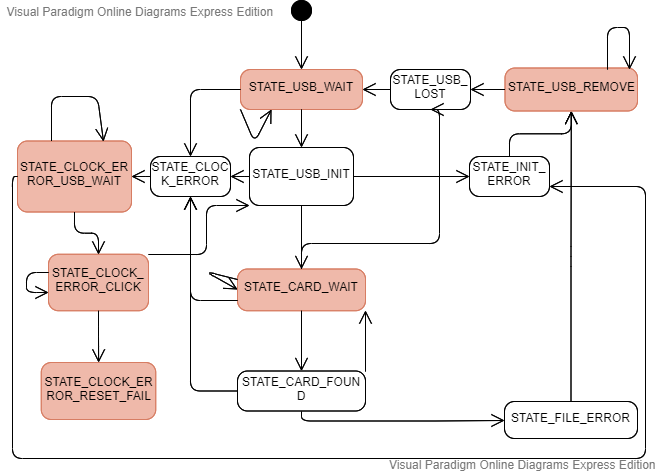
\includegraphics[scale=0.6]{state_machine.png}
\end{figure}

\subsection{Napotkane problemy}
\subsection{Testowanie}
\subsection{Inne koncepcje}
\section{Menadżer obecności - umożliwiający katalogowanie daych}
\section{Baza studentów - umożliwiająca identyfikakację danyc hzebranych z ELS}

\indent Zaproponowane przeze mnie rozwiązanie składa się z dwóch części:
\begin{enumerate}
\item Urządzenia opartego o platformę Arduino rozszerzoną o dodatkowe moduły niezbędne do odczytania potrzebnych informacji
\begin{itemize}
\item Moduł RFID - odczytujący unikalny identyfikator z legitymacji studenckiej
\item USB Host Shield - pozwalający na podłączenie zewnętrznej pamięci do Arduino i zapisanie zebranych informacji
\item Wyświetlacz LCD + Buzzer - pozwalający na komunikację z użytkownikiem
\item Zegar czasu rzeczywistego
\end{itemize}
\item Aplikacji internetowej pozwalającej na tworzenie i zarządzanie wykładami. Portal umożliwia utworzenia własnego użytkownika, do którego można przypisywać zajęcia, w ramach których można rejestrować obecności studentów
zebrane przy pomocy opisanego wyżej urządzenia.
\end{enumerate}

\chapter{Realizacja}
\chapter{Możliwości rozwoju}
\begin{itemize}
\item dostęp do usos i propagowanie zebranych danych na stronach uczelnianych
\item Udostępnienie systemu dla studentów i umożliwienie monitorowania swoich obecności (logowanie tylko przez uczelnianego maila, albo konta utworzone wyłącznie przez administratora)
\item powiadomienia mailowe do studenta o zbliżającym się wyczerpaniu limitu nieobecności
\end{itemize}

\chapter{Problemy}
\chapter{Wnioski}

\ldots

%%%%% BIBLIOGRAFIA

%\begin{thebibliography}{1}
%\bibitem{example} \ldots
%\end{thebibliography}

\end{document}


